\section{Lecture 6: Sampling Theorem}



\subsection{Introduction}
Sampling is broadly defined as the process of taking samples of an analog signal so as to convert it to a digital sequence. Sampling is the fundamental process that converts analog signal to digital signal. 

\begin{figure}[ht]
\centering
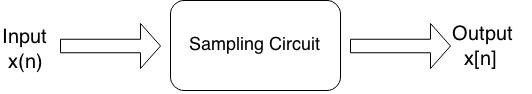
\includegraphics[width=0.5\textwidth]{block_1_.jpg}
\caption{\label{fig:}Block Diagram of a Sampling System.}
\end{figure}



One of the best examples of application of  sampling could be that of an Analog to Digital Converter (ADC). An ADC continuously take samples of the incoming data and gives an output as a sequence of discrete signals.  

The audio CDs that we play on our music systems are recorded by continuous sampling of the incoming audio signal (music) and are written on to the CD as a sequence of Digital Data sequence.



\begin{figure}[h]
 
\begin{subfigure}{0.5\textwidth}
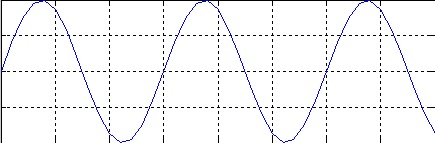
\includegraphics[width=0.9\linewidth, height=4cm]{continuous.jpg} 
\caption{Continuous Sine Wave}
\label{fig:subim1}
\end{subfigure}
\begin{subfigure}{0.5\textwidth}
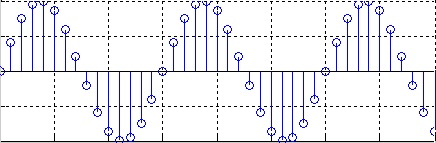
\includegraphics[width=0.9\linewidth, height=4cm]{discrete.jpg}
\caption{Discrete Sine Wave}
\label{fig:subim2}
\end{subfigure}
 
\caption{Sampling of a Continuous Sine Wave}
\label{fig:image2}
\end{figure}


\subsection{Sampling Theorem}
Also known as "Shannon-Whittaker-Nyquist theorem on Sampling".

When a signal is sampled, there is a possibility to lose information. During the sampling process, a lot of unwanted information maybe clubbed with the actual useful data.There is a need to filter out the unwanted part or the 'imposters' created by sampling.

Considerations for a given signal x(t):
\begin{enumerate}
\item The signal has a Fourier Transform.
\item The Fourier Transform is non-zero up to a maximum finite frequency $'f_m'$.
\end{enumerate}

The sampled signal is sampled at a frequency $'f_s'$.

The Sampling Theorem can be stated as:

A band-limited signal, band-limited to a maximum frequency $f_m$ can be perfectly reconstructed from it's samples taken at a rate $f_s=\frac{1}{T_s}$, such that $f_s>2f_m$ .

\subsection{Proof}


Sampling is a linear process.

Net consequence of a sampling spectrum is given by the sum of contributions by individual spectral pieces.

Consider a signal x(t), with Fourier Transform X(f).

The signal will be sampled at a frequency at a frequency $f_s$.

The Nyquist sampling theorem states that for the complete reconstruction of a signal, the sampling frequency $f_s>2f_m$.

If $f_s<2f_m$, the 'imposters' created by sampling will cloud with the original signal. Thus, resulting in loss of data. 

$f_s>2f_m$ implies $f_s-f_m>f_m$.

The imposter frequency varies from $f_s$ to $f_s-f_m$.

The Nyquist criteria ensure that since $f_s-f_m>f_m$, the imposter frequency does not mic with the actual data.

Thus, reconstructing the entire signal is basically filtering out all the 'imposters' created and only obtain the original signal.

\paragraph{}
The process of sampling will be further discussed in the next session.






